\documentclass[11pt]{article}
\usepackage[margin=1in]{geometry}
\usepackage[T1]{fontenc}
\usepackage[utf8]{inputenc}
\usepackage{lmodern}
\usepackage{microtype}
\usepackage{booktabs}
\usepackage{longtable}
\usepackage{tabularx}
\usepackage{array}
\usepackage{graphicx}
\usepackage{amsmath,amssymb}
\usepackage{enumitem}
\usepackage[dvipsnames]{xcolor}
\usepackage[round,authoryear]{natbib}
\usepackage[colorlinks=true,allcolors=MidnightBlue]{hyperref}
\usepackage[nameinlink,noabbrev]{cleveref}
\usepackage{tikz}
\usetikzlibrary{arrows.meta,positioning,fit}
\usepackage{caption}
\usepackage{subcaption}
\usepackage{fancyhdr}
\setlength{\headheight}{14pt}

% Generated/checked against results/final_synthesis after the ORCHARD run.
\newcommand{\SourceN}{2,321}
\newcommand{\SourceClusters}{12}
\newcommand{\TermN}{312}
\newcommand{\TermClusters}{12}
\newcommand{\TermEligible}{494}
\newcommand{\HFBlockN}{138}
\newcommand{\HFBlockK}{4}
\newcommand{\LeanBlockN}{27}
\newcommand{\LeanBlockK}{3}


\definecolor{human}{HTML}{1F5A85}
\definecolor{machine}{HTML}{8E3B46}
\definecolor{soft}{HTML}{F2F5F7}
\newcolumntype{Y}{>{\raggedright\arraybackslash}X}
\newcommand{\code}[1]{\texttt{#1}}
\newcommand{\xmin}{x_{\min}}
\newcommand{\caution}[1]{\textcolor{machine}{\textbf{#1}}}

\pagestyle{fancy}
\fancyhf{}
\lhead{Proof certificates, cognition, and mathematical uptake}
\rhead{August 2026}
\cfoot{\thepage}

\title{\textbf{From Proof Certificates to Mathematical Uptake}\\
\large A Critical Reanalysis and Multiscale Research Program for AI-Generated Mathematics}
\author{Research synthesis building on Viteri and DeDeo (2022)}
\date{1 August 2026}

\begin{document}
\maketitle

\begin{abstract}
AI systems increasingly produce kernel-checked formal proofs, but correctness is only one
property of a mathematical contribution.  This report critically audits a large exploratory
extension of \citet{viteri2022}, recovers the exact source of an apparent power-law
discrepancy, repairs paired analyses, and develops a research program connecting proof
networks to cognitive science, philosophy of mathematical practice, and AI for mathematics.
The original 2022 power-law pipeline fixed $\xmin=10$; the newer pipeline selected $\xmin$
by Kolmogorov--Smirnov optimization.  The estimates therefore measure different portions of
the degree distribution.  The defensible invariant is heavy-tailed reuse, not a universal
pure power law or a cutoff-free exponent.

In \SourceN{} same-statement human/AI Lean-script pairs from \SourceClusters{} coarse source
groups, AI scripts contain more local decomposition (median \code{have}: 3 versus 6;
median paired difference $+1$) while strict and loose source-level premise heuristics have
median paired difference zero.  A new elaborated-term analysis retains \TermN{} of
\TermEligible{} paired graphs after excluding either member if Lean error recovery introduced
\code{sorryAx} or \code{SyntheticOpaque}.  AI terms are modestly larger in the pair-weighted
analysis (median paired $+290$ nodes), although equal-source uncertainty includes zero; they are
slightly deeper and have a lower constant-node share.  Their apparent heavier
reuse tail at low cutoffs disappears at the publication convention $\xmin=10$.
Under the published belief dynamics, theorem belief shows no paired difference at any tested
error rate: the median paired difference is zero for $\epsilon\in\{.10,.05,.01\}$.
These results support a narrow hypothesis: current AI proof production often adds internal
scaffolding without clearly expanding the named library interface.  They do not establish
that AI uses less mathematical knowledge, produces epistemically inferior mathematics, or
has a universal proof-network signature.

The central proposal is a four-scale framework separating (i) kernel-checkable derivation,
(ii) human-facing proof presentation, (iii) library-level reuse and maintenance, and
(iv) social uptake and trust.  It yields preregisterable experiments in which proof content,
presentation, authorship labels, and optimization objectives are independently manipulated.
\end{abstract}

\section{Executive assessment}

The prior work is ambitious and contains real discoveries, especially its willingness to
falsify its own early claims.  Its strongest contribution is not a single scalar measure of
``AI mathematical style.''  It is a set of contrasts that reveal why such a scalar is unlikely
to exist.  Proof scripts, elaborated proof terms, declaration graphs, generated certificate
stores, and the dynamics of a human reader are different objects.  Treating them as
interchangeable made several early findings look stronger and more unified than the evidence
allows.

After repair, four conclusions remain.

\begin{enumerate}[leftmargin=*,itemsep=.35em]
  \item \textbf{The power-law discrepancy has an exact provenance.}  The archived publication
  script set \code{cutf=10} and called \code{powerlaw.Fit(..., xmin=cutf)}.  The later
  automatic fit commonly chose $\xmin\approx1$.  Neither estimate is intrinsically wrong, but
  they are not interchangeable.
  \item \textbf{The paired source evidence is about decomposition, not library avoidance.}
  Same-statement AI scripts use more \code{have} statements.  Once comments and strings are
  stripped, the claimed premise gap vanishes under both loose and strict regex definitions.
  \item \textbf{Elaborated terms add a second, non-regex signal.}  In the clean paired subset,
  AI proof terms tend to contain more internal nodes and edges and contain a smaller fraction of
  constant nodes.  The size interval crosses zero after giving each source group equal weight,
  while the constant-share contrast remains directional.  This is compatible with additional
  local scaffolding.  It is not equivalent to
  lower mathematical sophistication or weaker understanding.
  \item \textbf{Macro-level contrasts remain descriptive.}  A generated certificate layer
  designed to be terminal will naturally have few later citations.  Comparing it to a
  maintained human library confounds authorship with artifact role, chronology, and design
  objective.  Such cases motivate hypotheses but do not identify an authorship effect.
\end{enumerate}

\noindent The appropriate successor project should therefore ask: \emph{which production
objectives generate which proof artifacts, and how do those artifacts affect human validation,
understanding, reuse, and repair?}  This question is simultaneously computational, cognitive,
and philosophical.

\section{What was fixed, and what still required repair}

Claude's revision correctly withdrew several headline claims.  In particular, it stopped
interpreting a non-significant difference as equality, stripped comments and strings before
counting premise-like tokens, narrowed a rank calculation to its selected block, and replaced
overlapping one-way sums of squares with a nominally joint model.  These are substantive
improvements.  The audit nevertheless found additional defects summarized in
\cref{tab:audit}.

\begin{table}[p]
\centering
\caption{Audit of the revised analysis.  ``Resolved here'' means that the final synthesis
either corrects the code or withdraws the affected inference.}
\label{tab:audit}
\small
\begin{tabularx}{\textwidth}{p{.18\textwidth}Y Y}
\toprule
Issue & Why it matters & Resolution in this report \\
\midrule
Power-law cutoff & Automatic KS selection and fixed $\xmin=10$ estimate different tails. &
Recovered the archived production code; report a cutoff sweep and model-family caveat. \\
Premise regex & Capitalized or dotted source tokens are not authoritative elaborated dependencies. &
Use regex results only as script-interface proxies; add elaborated constant-node measures. \\
``TOST-style'' label & Percentile-CI containment inside a post hoc $10\%$ margin is not a formal TOST. &
Call it a descriptive smallest-effect-size-of-interest check; do not claim established equivalence. \\
Variance bootstrap & Each row, rather than each resampled theorem instance, received a new pseudo-problem label, producing zero-width CIs. &
Correct the relabeling; for complete blocks use an exact theorem/system/residual sum-of-squares partition on $\log(1+y)$. \\
HF complete-block search & Forty random triples among 45 systems missed large valid blocks. &
Exhaustively seed all triples; recover a \HFBlockN$\times$\HFBlockK{} complete block. \\
Stale report sections & Corrected results coexisted with old 7-system ranks and overlapping 89.8\%+16.4\% variance claims. &
Treat the old Markdown as an exploratory lab notebook, not a citable final report. \\
Lean error recovery & Many extracted graphs contained \code{sorryAx}/\code{SyntheticOpaque}; these are not completed proofs. &
Exclude a pair if either graph contains either label; disclose 312/494 retention. \\
Term truncation flag & \code{term0} uses zero expansion levels, leaving a constant frontier and marking every graph ``truncated.'' &
Interpret \code{term0} as the unexpanded root proof-term DAG; ignore that flag as an attrition indicator. \\
Belief simulations & The original expanded-graph run ended at 125/157 and wrote no final result; graph means can also mix isolates with connected nodes. &
Replace it with an incremental, component-aware run on all 312 clean \code{term0} pairs; report theorem belief separately and retain the model-validity caveat. \\
ETP provenance & A shortest Dijkstra path is one arbitrary certificate among possible paths; generated outputs are terminal by design. &
Downgrade causal language and propose randomized retention/organization experiments. \\
\bottomrule
\end{tabularx}
\end{table}

The most important meta-level correction is epistemic: a long exploratory pipeline should not
end by selecting only analyses that fit one narrative.  The report's reversals are scientifically
valuable, but they imply that future work needs frozen estimands, data-exclusion rules, and a
distinction between confirmatory and exploratory stages.

\clearpage

\section{Foundations: four objects, four scales}

\subsection{Why kernel correctness is not the whole object}

A Lean kernel checks whether a proof term inhabits a type.  This is an extraordinarily strong
guarantee about formal derivability, conditional on the statement, definitions, axioms,
elaborator, kernel, and computing stack.  It does not by itself tell us whether the formal
statement faithfully expresses the intended theorem, whether a human can see the proof's main
idea, whether its lemmas will be reused, or whether the artifact is easy to repair.  Recent formal
AI systems exploit precisely this grounded verification signal \citep{yang2023,hubert2026,ren2025};
that makes these other questions more urgent, not less important.

The philosophy of mathematical practice has long resisted identifying ordinary proof with a
bare formal derivation.  \citet{rav1999} emphasizes that proofs carry methods and mathematical
knowledge beyond their concluding propositions.  Work on explanation distinguishes correctness
from unification, dependence, and the revelation of a result's characteristic structure
\citep{mancosu2008}.  Rigour itself has been analyzed as plural and practice-sensitive
\citep{hamami2021,tanswell2024}, while fallibilist accounts locate justification partly in a
community's capacity to expose and correct errors \citep{detoffoli2021}.  Formalization changes
this ecology, but does not erase it \citep{avigad2023,avigad2024,detoffoli2026}.

\subsection{The proposed multiscale map}

\begin{figure}[ht]
\centering
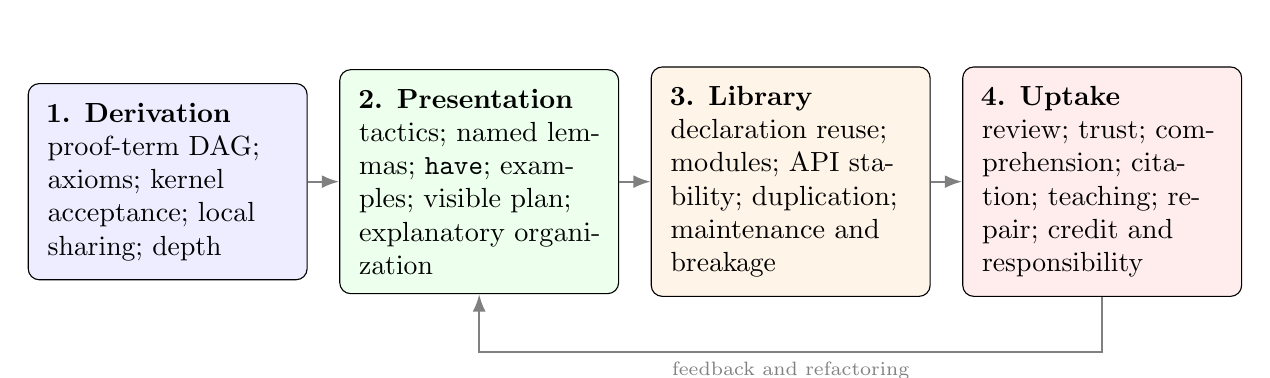
\begin{tikzpicture}[
  box/.style={draw,rounded corners,align=left,text width=3.05cm,minimum height=2.25cm,inner sep=7pt},
  arr/.style={-{Latex[length=2.2mm]},thick,gray}, node distance=4mm]
\node[box,fill=blue!7] (micro) {\textbf{1. Derivation}\\proof-term DAG; axioms; kernel acceptance; local sharing; depth};
\node[box,fill=green!7,right=of micro] (meso) {\textbf{2. Presentation}\\tactics; named lemmas; \code{have}; examples; visible plan; explanatory organization};
\node[box,fill=orange!9,right=of meso] (macro) {\textbf{3. Library}\\declaration reuse; modules; API stability; duplication; maintenance and breakage};
\node[box,fill=red!7,right=of macro] (social) {\textbf{4. Uptake}\\review; trust; comprehension; citation; teaching; repair; credit and responsibility};
\draw[arr] (micro.east) -- (meso.west);
\draw[arr] (meso.east) -- (macro.west);
\draw[arr] (macro.east) -- (social.west);
\draw[arr] (social.south) -- ++(0,-7mm) -|
  node[pos=.25,below,font=\scriptsize]{feedback and refactoring} (meso.south);
\end{tikzpicture}
\caption{A proof artifact moves through rendering, integration, and use across distinct scales;
later uptake can prompt feedback and refactoring.  Arrows are empirical processes, not logical
equivalences.  The same kernel term can be presented in different ways, and the same presentation
can receive different social treatment.}
\label{fig:scales}
\end{figure}

The 2022 epistemic-phase-transition (EPT) model concerns a hypothetical reader's changing beliefs
over a dependency network \citep{viteri2022}.  It is best interpreted as a model of reception or
justification under local uncertainty.  It is not an objective quality function for machine
corpora.  A verifier can collapse one kind of uncertainty while leaving statement correspondence,
explanatory understanding, provenance, and social responsibility unresolved.  Empirical studies
support this broader view: mathematicians validate using formal, informal, and example-based
reasoning \citep{weber2008}; experts attend more to logical structure and implicit warrants than
novices \citep{inglis2012,panse2018}; and mathematicians often read published proofs for insight
rather than line-by-line correctness \citep{mejiaramos2014}.  Interactive evaluations of language
models likewise find that users ask why a step was taken, not only whether the final answer is
right \citep{collins2024}.

\section{The power-law discrepancy, resolved}

The archive at \code{/Users/simon/Desktop/OLDER\_RESEARCH\_ARCHIVE/SCOTT} contains the script that
fed the reported table.  In \code{pl.py}, the operative lines are:
\begin{verbatim}
cutf=10
fit=powerlaw.Fit(data[0][1:], discrete=True,
                 xmax=data[0][0], xmin=cutf)
\end{verbatim}
The production file \code{convert\_final\_check.rb} writes the node count and nonzero reuse degrees
to \code{TEMP/data.dat}, invokes \code{./pl.py}, and prints the resulting exponent.  The independent
archive file \code{proof\_dist.rb} also begins with \code{xmin=10}.  This is direct provenance, not
an inference from approximate numerical matching.

The later Python analysis used the standard \code{powerlaw} behavior of choosing $\xmin$ to minimize
a KS distance.  It often chose a cutoff near one.  Fixed $\xmin=10$ reproduces 40 of 47 archived
exponents within 0.010; automatic estimates have essentially no cross-network correlation with the
published numbers.  This behavior is unsurprising.  Tail inference depends strongly on where the
tail begins, and model checking requires goodness-of-fit and comparisons to alternatives
\citep{clauset2009,alstott2014}.  In the recovered networks, a power law consistently beats an
exponential, but a lognormal is frequently competitive.  Strong scale-free claims therefore exceed
the evidence \citep{broido2019}.

The revised conclusion is:
\begin{quote}
Proof dependency networks exhibit heavy-tailed reuse.  A fixed-cutoff index near two summarizes
the degree tail under the publication convention, but no cutoff-free or universally pure power-law
mechanism has been established.
\end{quote}

This also changes how authorship comparisons should be interpreted.  An exponent difference at
$\xmin=2$ that disappears at $\xmin=10$ is evidence of different moderate-degree structure, not a
robust difference in the far reuse tail.

\section{Data and confirmatory estimands}

\subsection{Same-statement proof scripts}

The corrected NuminaMath analysis contains \SourceN{} pairs for which both a human and prover proof
were marked valid and both yielded at least one premise-like token under the extraction rule.
Pairs fall into \SourceClusters{} coarse source groups.  Metrics are line count, tactic count,
\code{have} count, and two source-token proxies for premise contact: a loose set of dotted or
capitalized identifiers and a strict set of dotted identifiers after comments and strings are
removed.  These are presentation metrics; neither token count is a semantic premise census.

The primary descriptive estimand is the median within-pair difference.  Uncertainty is reported
both by resampling pairs and by resampling source groups.  Because the latter estimand can still be
dominated by a large source, the final output also reports an equal-source summary: calculate each
source's median paired difference, then take the median across sources.  With only 12 source groups,
all cluster-level inference is necessarily coarse.

\subsection{Same-statement elaborated proof terms}

For a 500-pair extraction sample, both human and AI \code{term0} graphs existed for 494 statements.
The graph is the DAG of the theorem type and elaborated root proof term, with structurally identical
expressions deduplicated and edges directed from a child premise to the containing expression.  It
does not recursively expand referenced theorem definitions.  A pair is excluded if either graph
contains a label matching \code{sorry} or \code{SyntheticOpaque}; \TermN{} pairs remain.  This
36.8\% pairwise exclusion is substantial, and the retained sample must not be treated as a random
draw from all valid proofs.

Metrics include nodes, edges, longest DAG path, expression-sharing ratio, maximum out-degree,
out-degree Gini coefficient, constant-node count and share, and fixed-cutoff discrete tail-index
approximations.  Node and edge counts include both the theorem's type and value under a virtual root;
they are structural sizes, not human proof lengths.  Constant nodes are elaborated references, but
their number can still depend on elaboration and tactic expansion.

\subsection{Matched theorem-by-system blocks}

For the lean-eval records, ranking is performed only after selecting a complete
\LeanBlockN$\times$\LeanBlockK{} theorem-by-system block.  For the HuggingFace census, exhaustive
triple seeding and greedy enlargement recover a \HFBlockN$\times$\HFBlockK{} block that the earlier
random search missed.  Friedman tests and Kendall's $W$ quantify stable rank ordering within each
block.  A two-way sum-of-squares partition on $\log(1+y)$ attributes descriptive variation to
theorem, system, and residual/interaction; these shares sum exactly to one.  They do not estimate a
universal causal authorship effect because system identity, benchmark, decoding, and data lineage
remain entangled.

\section{Results}

\subsection{Source scripts: more local decomposition, no surviving premise gap}

\begin{table}[!htbp]
\centering
\caption{Corrected same-statement source results.  Intervals resample coarse source groups while
retaining their observed sizes.  P-values from thousands of pairs are not treated as measures of
substantive importance.}
\label{tab:source}
\small
\setlength{\tabcolsep}{4pt}
\begin{tabular}{lrrrr}
\toprule
Metric & Human median & AI median & Median paired $\Delta$ & Source-cluster 95\% interval \\
\midrule
Lines & 23 & 26 & $+2$ & $[1,3]$ \\
Tactic invocations & 12 & 11 & $0$ & see machine-readable supplement \\
\code{have} steps & 3 & 6 & $+1$ & $[0,1]$ \\
Loose premise proxy & 5 & 4 & $0$ & $[0,0]$ \\
Strict dotted proxy & 3 & 2 & $0$ & $[0,0]$ \\
\bottomrule
\end{tabular}
\end{table}

\begin{figure}[ht]
\centering
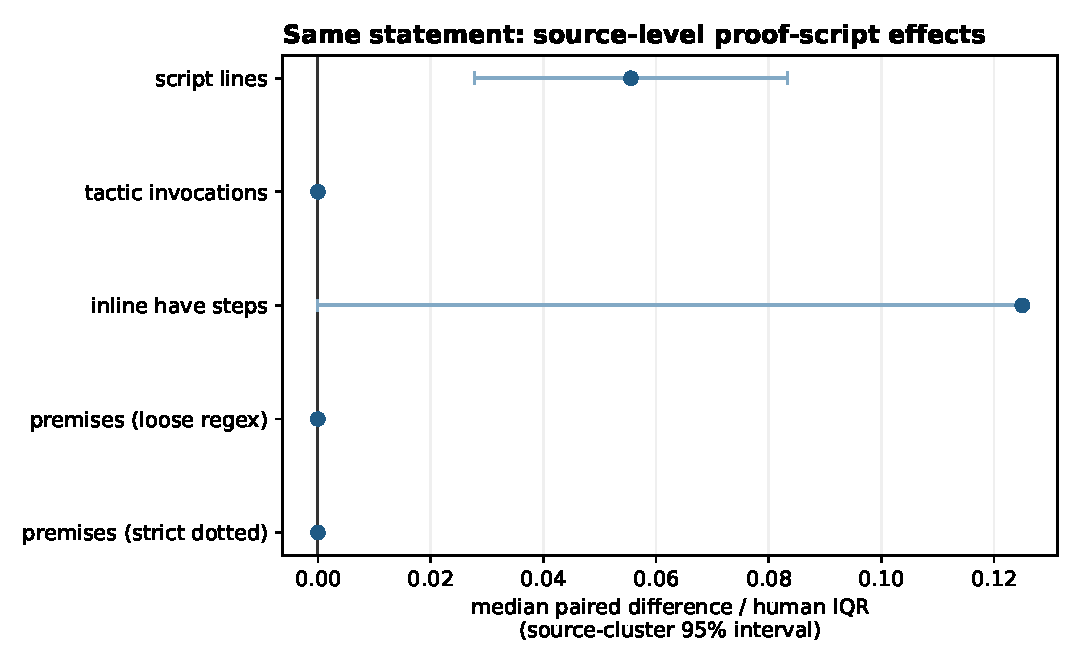
\includegraphics[width=.78\textwidth]{figures/paired_source_effects.pdf}
\caption{Paired source effects standardized by the human interquartile range.  A zero-width
interval can arise for discrete medians and 12 coarse clusters; it should not be read as literal
certainty or as a formal equivalence result.}
\label{fig:source}
\end{figure}

The line-count difference is small relative to the distribution, but calling the proofs ``the
same length'' requires a justified equivalence margin.  The previous $\pm10\%$ margin was generated
from the human median after the fact and its CI-containment procedure was not formal TOST.  The
responsible conclusion is simply that the typical difference is a few lines in this corpus.

The \code{have} result is the most interesting surviving presentation contrast: the AI median is
twice the human median, even though the median paired difference is only one because the
distribution is zero-inflated and skewed.  Giving every source equal weight yields a median
difference of $0.5$ and a bootstrap interval $[0,1.5]$, so the result is a tendency rather than a
universal signature.  In contrast, the original claim that AI touched roughly half as much of the
library was a
measurement artifact.  Removing comments and strings eliminates the paired gap under both token
rules.  The data therefore support finer visible decomposition, not reduced named-premise contact.

\subsection{Elaborated terms: more internal structure, similar far-tail exponent}

\begin{table}[!htbp]
\centering
\caption{Clean paired \code{term0} results ($n=\TermN$).  The listed intervals are source-cluster
bootstrap intervals from the audited run; all metrics are exploratory and correlated.}
\label{tab:term}
\small
\begin{tabular}{lrrrr}
\toprule
Metric & Human median & AI median & Median paired $\Delta$ & Source-cluster 95\% interval \\
\midrule
Nodes & 3,816.5 & 4,561 & $+290$ & $[20,512]$ \\
Edges & 7,145.5 & 8,632.5 & $+538.5$ & $[39,1{,}039]$ \\
Sharing ratio & 1.875 & 1.895 & $+0.0089$ & $[0.0047,0.0121]$ \\
DAG depth & 65 & 68 & $+1$ & $[0,3]$ \\
Maximum reuse & 197.5 & 207.5 & $+2$ & $[0,10]$ \\
Reuse Gini & .4333 & .4398 & $+.0030$ & $[.0012,.0052]$ \\
Constant-node share & .0530 & .0456 & $-.0046$ & $[-.0061,-.0028]$ \\
$\alpha$, $\xmin=2$ & 2.102 & 2.057 & $-.024$ & $[-.033,-.014]$ \\
$\alpha$, $\xmin=5$ & 2.330 & 2.303 & $-.028$ & $[-.031,-.011]$ \\
$\alpha$, $\xmin=10$ & 2.531 & 2.527 & $-.009$ & $[-.019,.013]$ \\
\bottomrule
\end{tabular}
\end{table}

\begin{figure}[ht]
\centering
\begin{subfigure}{.58\textwidth}
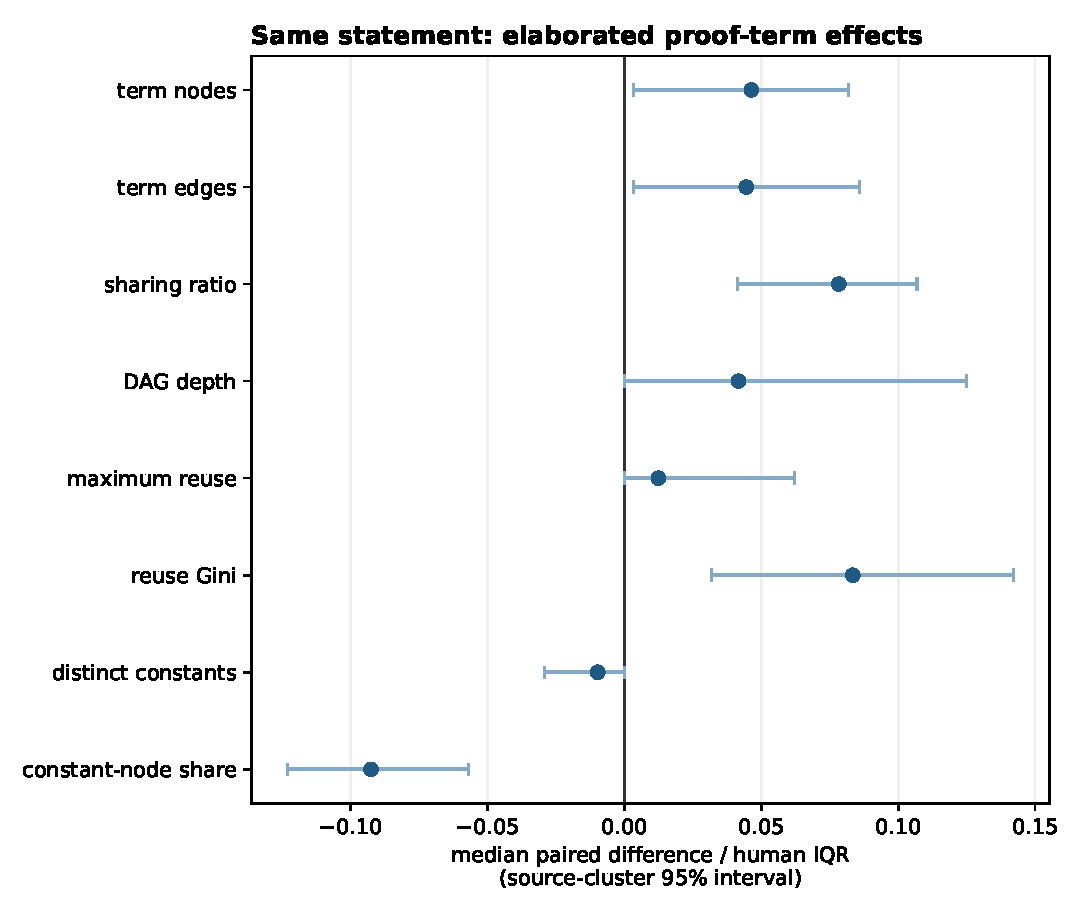
\includegraphics[width=\textwidth]{figures/paired_term_effects.pdf}
\caption{Structural paired effects.}
\end{subfigure}\hfill
\begin{subfigure}{.38\textwidth}
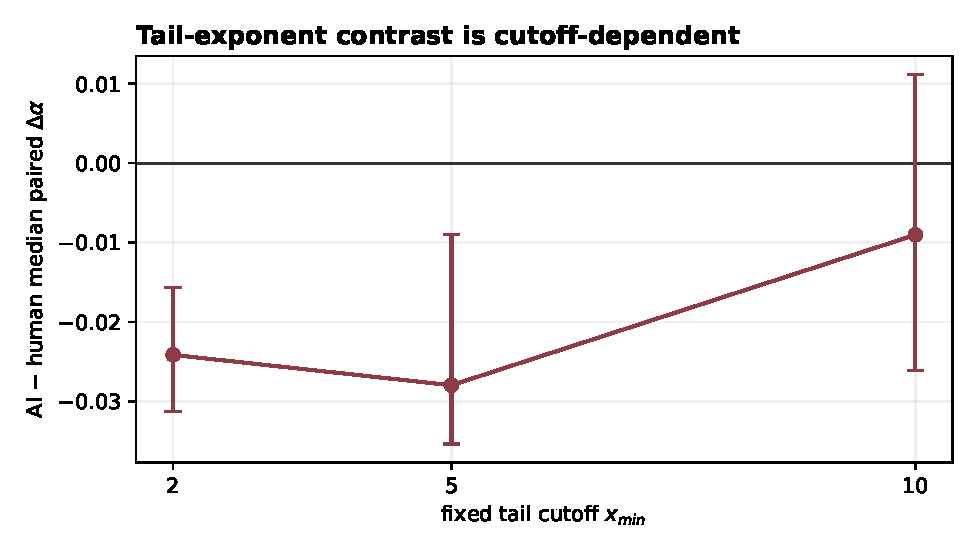
\includegraphics[width=\textwidth]{figures/alpha_sensitivity.pdf}
\caption{Tail-cutoff sensitivity.}
\end{subfigure}
\caption{Elaborated proof-term comparisons.  AI terms are larger and contain proportionally fewer
constant nodes.  The exponent contrast is present only when moderate-degree nodes enter the fit.}
\label{fig:term}
\end{figure}

The pair-weighted conjunction of source and term results suggests an \emph{internalization}
pattern: similar
visible contact with named premises, but more generated expression structure between those
interfaces and the theorem.  This pattern could arise from subgoal decomposition, explicit
coercions, normalization, repeated tactic templates, or different choices of theorem APIs.  It
does not establish which mechanism is operative.  Source-balanced intervals for nodes
$[-6.5,540.75]$ and edges $[-8,1025]$ cross zero, whereas the source-balanced constant-share
interval $[-.00624,-.00071]$ does not.  Thus proportional internal structure is more stable than
absolute size across the 12 coarse source groups.  A decisive follow-up should compare multiple
proofs elaborated under the same Lean/Mathlib version and decompose node counts by expression type,
tactic origin, and referenced declaration.

Most importantly, the low-cutoff exponent effect is not stable.  At $\xmin=10$, the paired median
difference is near zero and its interval crosses zero.  This aligns the paired AI comparison with
the recovered publication convention and prevents a narrative about universally heavier AI reuse
tails.

\subsection{Belief dynamics: structural differences do not create a theorem-belief deficit}

The unfinished expanded-term simulation was not simply resumed.  Expansion folds a variable amount
of Mathlib into each root proof and made the earlier 157-pair run prohibitively slow.  A redesigned
ORCHARD analysis applies the published asymmetric-Ising update to the same 312 clean, unexpanded
graphs used above, writes every pair incrementally, and distinguishes theorem belief, all-node mean,
and theorem-root-component mean.  Thirty-two Monte Carlo runs per graph are used in the final
sensitivity pass, with common seeds across each human/AI pair.

Every retained \code{term0} graph is one weak component: the theorem-root component share is 1.0.
Thus isolate conditioning is immaterial at this micro scale, although it remains essential for
source- and library-level graphs.  The 32-run sensitivity result is shown in
\cref{tab:belief}; its qualitative conclusion agrees with the earlier eight-run diagnostic.

\begin{table}[!htbp]
\centering
\caption{Paired belief dynamics on clean unexpanded terms.  Differences in all-node means are
smaller than $10^{-3}$ and should not be elevated by large-sample p-values.}
\label{tab:belief}
\small
\begin{tabular}{lrrrr}
\toprule
Error $\epsilon$ & Human theorem median & AI theorem median & Median paired $\Delta$ &
Median all-node $\Delta$ \\
\midrule
.10 & .9594 & .9578 & 0 & .00043 \\
.05 & .9747 & .9747 & 0 & .00050 \\
.01 & .9802 & .9828 & 0 & .00029 \\
\bottomrule
\end{tabular}
\end{table}

The model therefore predicts essentially the same epistemic outcome despite detectable structural
contrasts.  In fact, the tiny all-node differences favor AI terms, while theorem medians do not
differ.  The correct conclusion is negative: these proof-term differences do not support an AI
epistemic deficit under the 2022 dynamics.  This is a model implication, not behavioral validation
of the model.

\subsection{Matched systems: theorem effects are large, but style stability is dataset-specific}

The corrected deterministic lean-eval block gives Kendall $W=0.374$ for vocabulary ratio, $0.457$
for lines, $0.652$ for \code{have}, and $0.586$ for distinct-premise rank.  Thus the original
7-system rank
table was invalid, but rank stability does survive in a narrower 3-system block.  The recovered
HuggingFace block gives $W=0.534$, $0.050$, $0.121$, and $0.739$ for the same four
metrics, respectively.  Line and \code{have} stability do \emph{not} replicate, while premise and
vocabulary ordering are strong in this selected block.

In the HF block's exact $\log(1+y)$ partition, theorem accounts for 86.4\% of line-count variation,
system for 0.8\%, and interaction/residual for 12.8\%.  Distinct-premise count reverses that
balance: theorem accounts for 33.2\%, system for 56.6\%, and interaction/residual for 10.2\%.
The question ``problem or prover?'' therefore has a metric-specific answer even inside one block.

This reversal is informative.  ``Verbosity is a stable trait of a prover'' is not a corpus-free
law.  The HF block contains related dataset/model variants, and its result may reflect lineage or
decoding configuration as much as base-model identity.  The complete-block variance decomposition
in the supplement is therefore descriptive.  A credible variance-components claim requires a
crossed generation design in which every theorem is sampled repeatedly from every independently
defined system under a fixed toolchain and budget.

\subsection{Why the macro-corpus results remain hypotheses}

The Equational Theories Project (ETP) generated layer is an extreme and useful case: most generated
declarations are never cited, and the layer has low modularity when viewed alone.  But the artifact
is a certificate store built to settle implications, not a long-lived API designed for future
authors.  Its terminality is partly an objective, not necessarily a machine cognitive limitation.
Likewise, a Dijkstra-selected shortest provenance path does not identify ``the'' derivation when
many derivations are possible.

The belief-dynamics analyses raise a separate identification problem.  Mean belief over all nodes
is highly sensitive to isolates and graph boundary choices.  Comparing an explicit human layer to
a generated terminal layer without conditioning on connected status can turn data organization
into an apparent epistemic effect.  The completed component-aware \code{term0} analysis resolves
this concern only at the micro proof-term scale: all 312 retained graphs are connected to their
theorem roots and show no median paired theorem-belief difference.  It does not repair the
unconditioned macro comparison.  The macro results should therefore be retained as case studies
that motivate controlled interventions, not as evidence that machine mathematics is intrinsically
fragile, heap-like, or non-modular.

\section{Interpretation across cognitive science, philosophy, and AI}

\subsection{Cognitive science: model the reader, not only the artifact}

The EPT model offers a generative bridge from dependency structure and local uncertainty to global
confidence.  Its next test should collect belief trajectories from readers.  Structural metrics
alone cannot validate cognitive plausibility.  Expert proof reading involves backward looks,
implicit-warrant reconstruction, examples, prior authority, and goal-dependent allocation of
attention \citep{weber2008,inglis2012,mejiaramos2014,panse2018}.  These processes suggest measurable
extensions: node-specific priors, selective attention, chunking into lemmas, trust in authors or
verifiers, and stopping when expected checking value falls below its cost.

AI proofs are especially useful experimental stimuli because one kernel term can be transformed
into several presentations while correctness is held fixed.  A proof can be expanded or compressed,
renamed, reorganized into lemmas, supplied with examples, or labeled human/AI.  This enables causal
tests that historical proof networks cannot provide.

\subsection{Philosophy: correspondence, explanation, and repair}

Formal verification relocates rather than eliminates epistemic labor.  If the term checks, attention
moves to statement correspondence, definitions, axioms, imported libraries, and the provenance of
the formalization.  This is a correspondence problem between intended and formal mathematics.  It
also leaves explanation open: a proof may certify without displaying why a theorem depends on a
characteristic structure or how its method unifies other results \citep{mancosu2008,rav1999}.

A useful operationalization of mathematical justification is \emph{repair capacity}.  Can another
agent find the key dependency, locate a gap in an informal rendering, update the proof after an API
change, and explain the change?  This connects fallibilist correction \citep{detoffoli2021} to
software-like maintenance without reducing mathematics to software engineering.  It also avoids
the false choice between perfect formal certainty and merely social acceptance.

\subsection{AI for mathematics: optimize beyond pass rate}

Current formal systems demonstrate that verified search can reach Olympiad-level performance
\citep{trinh2024,hubert2026}, while retrieval and subgoal decomposition make premise access and
proof organization explicit design problems \citep{yang2023,ren2025}.  AI has also assisted human
discovery by exposing patterns that mathematicians turn into concepts and proofs
\citep{davies2021}.  These successes suggest a transition from proof scarcity to proof abundance.

If many valid certificates can be generated, the bottleneck becomes selection and presentation:
which proof should enter a library, which lemmas deserve names, what should a reviewer inspect, and
what artifact will teach or support future work?  Training only for kernel acceptance or short
tactic traces can produce locally efficient but socially expensive proofs.  A research program
should make those downstream costs visible to the objective.

\section{A significant research program}

\subsection{Work package 0: measurement validity and an open proof observatory}

Build a versioned extraction layer that records, for each generated proof:
\begin{itemize}[leftmargin=*]
  \item exact theorem statement, imports, Lean/Mathlib commit, options, axioms, and validation log;
  \item source syntax trees rather than regex tokens;
  \item elaborated proof terms with node type, constant identity, universe normalization policy,
        tactic provenance where available, and explicit error-recovery flags;
  \item declaration-level dependencies at the commit where the proof was produced;
  \item generator identity, prompt/search budget, samples attempted, wall-clock compute, and selection rule;
  \item links among informal problem, formal statement, source script, proof term, and later revisions.
\end{itemize}
Hand-audit a stratified sample and report precision/recall for premise extraction.  Unit tests should
include nested comments, quoted identifiers, namespaces opened locally, generated declarations,
multiple proof bodies, and intentional failure cases.  Publish hashes and manifests so a derived
table can be traced to immutable inputs.

\subsection{Work package 1: a genuinely crossed proof-production experiment}

Select 150--300 theorems stratified by domain, statement length, library depth, and difficulty.
For each theorem collect at least two independent human formalizations where feasible and three
independent samples from each of four contrasting AI architectures: whole-proof generation,
retrieval-augmented generation, interactive/agentic search, and RL-guided formal search.  Fix the
Lean/Mathlib version and expose the same accessible premises and budgets.

The primary model should be preregistered before generation:
\begin{equation}
  g(y_{t,s,r}) = \mu + A_s + T_t + (A\!\times\!D)_{s,d(t)} + u_{t,s} + \epsilon_{t,s,r},
\end{equation}
where theorem $t$, system $s$, repeat $r$, and domain $d$ are crossed; $g$ is specified in advance
(for counts, usually $\log(1+y)$ or a negative-binomial link).  Report theorem, system, interaction,
and repeat variance.  Hold out theorem families, not random near-duplicate statements.

Primary outcomes should be few and mechanistic: internal expression nodes per distinct constant,
named intermediate claims, proof-term depth, retriever recall, reuse concentration, and generated
lemma survival.  Power-law exponents are secondary sensitivity summaries with fixed cutoffs and
alternative-distribution tests.

\subsection{Work package 2: causal experiments on proof reception}

Use kernel-equivalent presentations in a factorial reader study:
\begin{center}
\begin{tabular}{ll}
\toprule
Factor & Levels \\
\midrule
Presentation & compressed / expanded / hierarchically chunked \\
Provenance label & human / AI / unlabeled (randomized, sometimes deceptive with debrief) \\
Verifier information & none / ``kernel checked'' / audit trail and assumptions \\
Error status & valid / planted local gap / statement-correspondence mismatch \\
Reader & advanced undergraduate / graduate / domain expert \\
\bottomrule
\end{tabular}
\end{center}

Measure confidence after each proof segment, validation accuracy, time, eye movements or navigation,
recall of the main idea, transfer to a nearby problem, calibration, and willingness to reuse a lemma.
Fit the EPT model to individual trajectories and compare it against sequential-evidence and
attention/chunking alternatives.  The key test is out-of-sample prediction: parameters inferred from
one set of proofs must predict confidence and error detection on held-out proofs.

\subsection{Work package 3: library uptake and maintenance}

Follow accepted human-, AI-, and mixed-authorship pull requests longitudinally.  Match or weight by
domain, project maturity, declaration type, size, review policy, and chronology.  Outcomes at 3, 6,
and 12 months should include citations by later declarations, number of downstream files, review
rounds, issue reports, API-breaking edits, proof repair time after dependency changes, and whether a
lemma is generalized, renamed, deprecated, or taught.

The strongest design is randomized assistance within a real library: route eligible contributions
to (i) ordinary generation, (ii) generation plus a library-architect agent optimizing reuse/API
quality, or (iii) generation plus a human editor.  All outputs remain human-reviewed.  This tests
whether apparent ``terminality'' is caused by machines, objectives, or editorial organization.

\subsection{Work package 4: an ecology of proof objectives}

Train or rerank proof agents under controlled multi-objective rewards:
\begin{align*}
R ={}& R_{\mathrm{valid}} - \lambda_1 C_{\mathrm{compute}}
      - \lambda_2 C_{\mathrm{repair}} + \lambda_3 U_{\mathrm{future}}\\
    &+ \lambda_4 H_{\mathrm{reader}} + \lambda_5 P_{\mathrm{provenance}},
\end{align*}
where future reuse $U$, human reception $H$, and provenance quality $P$ are measured on held-out
tasks rather than guessed from static proxies.  Compare Pareto fronts rather than collapsing all
values into one score.  A proof can be short but opaque, readable but redundant, or reusable but
expensive; those tradeoffs should remain visible.

\subsection{Work package 5: dialectical and adversarial mathematical agents}

Correctness filters do not guarantee that a formal statement is the intended one.  Pair a proposer
with independent agents assigned to statement auditing, counterexample search, dependency
minimization, proof explanation, and hostile review.  Preserve failed conjectures and objections as
first-class research objects, following the dialectical tradition in mathematical practice
\citep{corneli2018}.  Evaluate whether heterogeneous audit roles catch correspondence errors and
improve human calibration more efficiently than simply sampling more proofs from one prover.

\subsection{Preregistered hypotheses and falsifiers}

\begin{longtable}{p{.08\textwidth}p{.40\textwidth}p{.42\textwidth}}
\caption{A compact confirmatory agenda.}\label{tab:hypotheses}\\
\toprule
ID & Prediction & Decisive falsifier or boundary condition \\
\midrule
\endfirsthead
\toprule ID & Prediction & Decisive falsifier or boundary condition \\
\midrule
\endhead
P1 & At fixed theorem, toolchain, and accessible library, AI proofs have more internal expression
nodes per distinct referenced constant. & The system effect vanishes after tactic family and repeat
are crossed, or reverses in at least two independent architectures. \\
P2 & Increased \code{have} use mediates part, but not all, of the term-size difference. & A controlled
style intervention changes \code{have} count without changing term structure, or mediation fails on
held-out systems. \\
P3 & Chunking proof terms into meaningful named lemmas improves reader calibration and transfer more
than equal-length arbitrary chunking. & Arbitrary and meaningful chunking perform equivalently on
held-out proofs and experts. \\
P4 & A kernel-checked label reduces line-by-line checking but does not eliminate statement-audit
effort. & Verifier information changes neither navigation nor error detection, or suppresses both
local and correspondence-error detection equally. \\
P5 & Library-architect optimization increases later reuse and lowers repair cost without reducing
acceptance. & Randomized architecture assistance yields no improvement at 6--12 months or merely
inflates trivial citations. \\
P6 & Tail-exponent authorship differences are concentrated below $\xmin=10$ and are not stable across
toolchains. & A preregistered fixed-$\xmin=10$ contrast replicates across domains, systems, and
toolchain versions with alternative families rejected. \\
P7 & EPT parameters predict segment-by-segment confidence better after adding attention and chunking
than from graph structure alone. & A simple length/position baseline matches held-out predictive
performance, or fitted parameters fail to transport between proofs. \\
\bottomrule
\end{longtable}

\section{Standards for claims about AI-generated mathematics}

Future papers should state which of the following has actually been demonstrated:
\begin{enumerate}[leftmargin=*]
  \item \textbf{Formal validity:} a kernel checks a term under enumerated assumptions.
  \item \textbf{Correspondence:} experts agree that the formal statement and definitions match the
        intended mathematical claim.
  \item \textbf{Explanatory value:} readers identify why the result holds and transfer the method.
  \item \textbf{Library value:} the contribution forms a stable, reusable interface.
  \item \textbf{Social robustness:} provenance, review, responsibility, and correction mechanisms
        support warranted communal uptake.
\end{enumerate}
No single network statistic certifies all five.  The EPT model is most naturally linked to the fifth
through a model of readers, while proof terms strongly address the first.  The research opportunity
lies in measuring the transformations between them.

\section{Conclusion}

The corrected analyses do not reveal a universal architecture of machine mathematics.  They reveal
something more actionable: current AI and human proofs of the same statement can expose a similar
named-library interface while differing in internal scaffolding and presentation.  The difference is
modest, cutoff-sensitive, and strongly conditioned by corpus and extraction choices.  At library
scale, much larger contrasts often reflect what an artifact was built to do.

Viteri and DeDeo's central question---how finite, fallible agents come to trust long deductive
arguments---becomes sharper in the age of AI.  Kernel verification can make valid certificates
abundant, but it does not automatically create explanations, maintainable libraries, or calibrated
human understanding.  A mature science of AI-generated mathematics should therefore follow proofs
from derivation through presentation and integration to uptake.  The multiscale program above turns
that philosophical distinction into controlled experiments, longitudinal outcomes, and falsifiable
models.

\appendix
\section{Reproducibility and computational provenance}

The final synthesis script is \path{code/final_synthesis.py}.  It consumes four compact tables:
\path{paired_numina_corrected.csv}, the clean paired \path{term0.csv},
\path{matched_hf_records.csv.gz}, and the lean-eval records.  The audited term extraction is in
\path{code/paired_term_structure.py}; corrected block and bootstrap routines are in
\path{code/matched_stats.py}.  The confirmatory resampling run used 10,000 bootstraps and 10,000
permutations on the CMU ORCHARD cluster, submitted as Slurm job 128378 (completed in 7m58s using
eight allocated CPUs; peak recorded RSS 700,868 KiB).  Inputs were transferred as a
728 KiB archive with SHA-256
\texttt{f779f00a0656a24bf8e7e12c98be6c96}\allowbreak
\texttt{4fb4071be4d3e88b90b30b62f2f8efeb}.  The returned result
archive verified against SHA-256
\texttt{cac276075ec55b8cfc25ca6cafb91549}\allowbreak
\texttt{d8beef824914df5b9a42fdf8203f7f43}.

The belief analysis is implemented in \path{code/paired_belief_term0.py}.  The 312 paired graph
inputs were transferred to ORCHARD with SHA-256
\par\noindent
\texttt{d0100b65be314d1d8466328a27cdfe0d}\allowbreak
\texttt{b8e53417e0cd03a9adec91eae777bc1f}.  Slurm job 128433 ran the eight-run diagnostic; job
128465 ran the 32-run sensitivity analysis (completed in 1m00s; peak recorded RSS 1,149,304 KiB).
The final returned archive has SHA-256
\par\noindent
\texttt{d7b168c956c6216da5e885afa65f3ec7d}\allowbreak
\texttt{c70b1b596e1cdb4300ca251b4151bfc}.

Bulk corpora and extracted networks remain on remote storage and are not embedded in the repository.
This limits third-party end-to-end reproduction.  A publication package should deposit immutable
paired graph samples, manifests, extraction logs, and licenses in an archival repository.

\section{Interpretive guardrails}

\begin{itemize}[leftmargin=*]
  \item The paired script sample requires at least one regex-counted premise in each proof and is
        not the same population as the paired term sample.
  \item The term sample has high pairwise exclusion due to error-recovery labels.  Exclusion can be
        associated with proof complexity or syntax, so effect sizes may be selected.
  \item ``Human'' and ``AI'' labels are dataset provenance labels, not pure causal treatments;
        human editing, retrieval, and multi-model pipelines blur the categories.
  \item Source groups are coarse and only 12 in number.  Cluster intervals have limited resolution.
  \item All term metrics share nodes and edges and are strongly dependent; no multiple-testing
        narrative should count them as independent replications.
  \item Tail-index approximations require at least 20 observations above a cutoff; results at
        different cutoffs have different samples as well as different estimands.
  \item The belief model is a theoretical cognitive mechanism.  Reproducing one published output
        does not behaviorally validate its update rule, priors, node ontology, or reading process.
\end{itemize}

\bibliographystyle{plainnat}
\bibliography{references}

\end{document}
